

\section{Tervezés}

\subsection{Bevezető}

Ebben a részben elsőként leírom, illetve összehasonlítom a multimédia üzenetküldő rendszer megvalósítási lehetőségeit, majd az általam kiválasztott módszer funkcionális egységeit,  részletesen tárgyalva azok szerepét és egymással való kapcsolatát.

\subsection{A megvalósítási lehetőségek}

Nézzük meg, hogy az IMS használata esetén milyen lehetőségek kínálkoznak a csoportos üzenetküldés megvalósítására. A megoldási lehetőségek ismertetése során kitérek azok előnyeire, hátrányaira, illetve a felmerülő problémákra.

\subsubsection{SIP MESSAGE üzenetek használata}
\label{sec:sip_message}

Első megoldásként kézenfekvőnek tűnhet, hogy a SIP protokoll által nyújtott MESSAGE típusú üzenet törzsében küldjük el a multimédia üzenetet a címzetteknek. Ennek a megoldásnak az az előnye, hogy nem kell másik protokollt használni az üzenetek átviteléért, hanem a SIP protokoll nyújtotta funkciókat alkalmazzuk. A megoldás előnye viszont eltörpül a hátrányok mellett. Először is a MESSAGE típusú üzenetnek nem adható meg egynél több címzett, így minden címzettnek különálló MESSAGE üzenetben kellene elküldeni ugyanazt a tartalmat. Ez a megszorítás redundanciához vezet, mivel a feladónak ugyanazt az üzenetet minden címzettnek külön-külön el kell küldenie, ami a válaszidőt is jelentősen megnöveli. Erre a problémára megoldást jelenthet, ha az üzenetet egy alkalmazás szerveren keresztül küldjük, ahol a szerver feladata az üzenet továbbítása az a címzetteknek. Ebben az esetben a feladó és a szerver között csak egyszer kerülne átküldésre az üzenet, ami a szűkebb sávszélességű felhasználói hálózatok esetén hatalmas előnyt jelent a többszörös küldéshez képest. Ahhoz, hogy ez a megvalósítás működhessen, a felhasználókból csoportokat kell létrehozni, és a MESSAGE üzenetet a címzettek URI-ja (Uniform Resource Identifier) helyett a csoport URI-jával címezni. Amikor az alkalmazás szerver megkapja ezt az üzenetet, a csoport azonosító alapján valamilyen módon -- pl. saját adatbázisból -- megkeresi azokat a felhasználókat, akik tagjai a csoportnak, és mindegyik csoporttagnak egyesével elküldi a kapott üzenet másolatát. Ebben az esetben szükség van az alkalmazás szerver oldalán egy olyan funkcióra, ami a csoportkezelést megvalósítja.
További problémát jelent, ha a küldött multimédia mérete meghaladja a MESSAGE üzenet törzsébe maximálisan megadható 1300 oktetet\footnote{RFC 3428 - Session Initiation Protocol Extension for Instant Messaging \cite{rfc3428}}. Ilyenkor a tartalmat a küldő oldalon kisebb darabokra kell tördelni, a darabokat külön üzenetekben elküldeni, majd a vevő oldalon a kisebb részekből a teljes üzenetet rekonstruálni. A probléma gyökere, hogy a SIP MESSAGE üzenettípus nem támogatja egy üzenet több darabban való átvitelét. A MESSAGE üzenet fejlécében nincs lehetőség olyan paramétert megadni, amiből a vevő egyértelműen el tudja dönteni, hogy a beérkező MESSAGE üzenetek közül melyik hordozza ugyanazon tartalom egy-egy darabját, és melyik nem, amiből következően rekonstruálni sem tudja azt. További gond, hogy az üzenetek nem sorszámozottak, így az eredeti küldési sorrendet sem tudnánk visszaállítani. Ezek a problémák abból fakadnak, hogy a MESSAGE üzenet használatát elsősorban rövid szöveges üzenetek továbbítására találták ki, és nem nagy multimédia tartalmakhoz. 
A megoldás hátrányainak sorát bővíti az is, hogy nem támogatott a késleltetett üzenetküldést sem. Utóbbi problémát -- hasonlóan a többszörös küldéshez -- orvosolhatnánk az alkalmazás szerver használatával, amely eltárolná azokat az üzeneteket, amelyek a nem elérhető címzetteknek mennek, és a szerver akkor kézbesítené azt, amikor a címzett elérhetővé válik.

{\color{red}(IDE MÉG RFC3428-ból PÁR DOLOG)
(Leírni még, hogy a vevők válasza többször jön, stb...)}

\subsubsection{Több címzettel rendelkező üzenetek használata}
\label{sec:mr_message}

Mint ahogy \aref{sec:sip_message}.~fejezetben láthattuk, a SIP specifikáció nem nyújt hatékony megoldást a több címzettű üzenetek továbbítására. Ebben az alpontban leírt megoldás abban tér el az előzőhöz képest, hogy az üzenet fejlécben lehetőség van több címzettet megadni. A folytatásban az ilyen típusú üzenetet több címzettel rendelkező, azaz MR (Multi Recipient) üzenetnek fogom nevezni. A több címzett megadásának a lehetősége jelentős előnyt jelent az alap SIP MESSAGE-et használó megoldáshoz képest. Először is, a feladónak elég csak egyszer elküldeni az üzenetet a CSCF felé, és nem annyiszor, ahány címzettje van az üzenetnek. Ez jelentősen lecsökkenti a hálózati erőforrások használatát. Másodszor, mivel a címzettek az MR üzenet fejlécében helyezkednek el, így az erre alkalmas hálózati szerverek a fejléc adatokat felhasználva képesek az üzeneteket hatékonyan eljuttatni az összes címzettnek anélkül, hogy az üzenet törzsét meg kellene vizsgálniuk. Tegyük fel, hogy a feladó hálózatában lévő S-CSCF, miután megkapja feladótól az MR üzenetet, annak minden címzettjére meghatározza az adott címzett felé vezető következő állomást (next hop CSCF), ahová továbbítani kell azt. Abban az esetben, ha kettő vagy több címzett esetén ugyanaz a next hop, akkor az S-CSCF abba az irányba MR üzenetként küldi tovább az üzenetet. Ha minden címzett next hop CSCF-je különbözik egymástól, akkor a szerver az egyes next hop-oknak hagyományos üzenetben küldi el annak egy-egy másolatát. Mivel a hálózatban található összes CSCF hasonlóan viselkedik, mint a feladót kiszolgáló S-CSCF, ezzel a módszerrel két szerver között ugyanaz az üzenet pontosan egyszer kerül átvitelre. Az üzenet terjedésének folyamatát \aref{fig:mrflow}.~ábrán követhetjük nyomon. Jól látható, hogy ezzel a módszerrel minden linken kizárólag egyszer küldjük át ugyanazt az üzenetet, ellentétben az aktuális IMS javaslattal, miszerint több címzett esetén egy linken többször kellene átküldeni ugyanazt az üzenetet (Például a III-as, IV-es és V-ös linken). Abban az esetben, ha egy olyan CSCF vesz egy MR üzenetet, amely nem képes MR üzeneteket kezelni, akkor a küldő CSCF felé hibaüzenetet küld. Ilyenkor a küldő CSCF újra elküldi az üzenetet hagyományos SIP üzenetként, minden címzettre külön-külön. 

\begin{figure}[htbp]
\center
\resizebox{10cm}{!}{
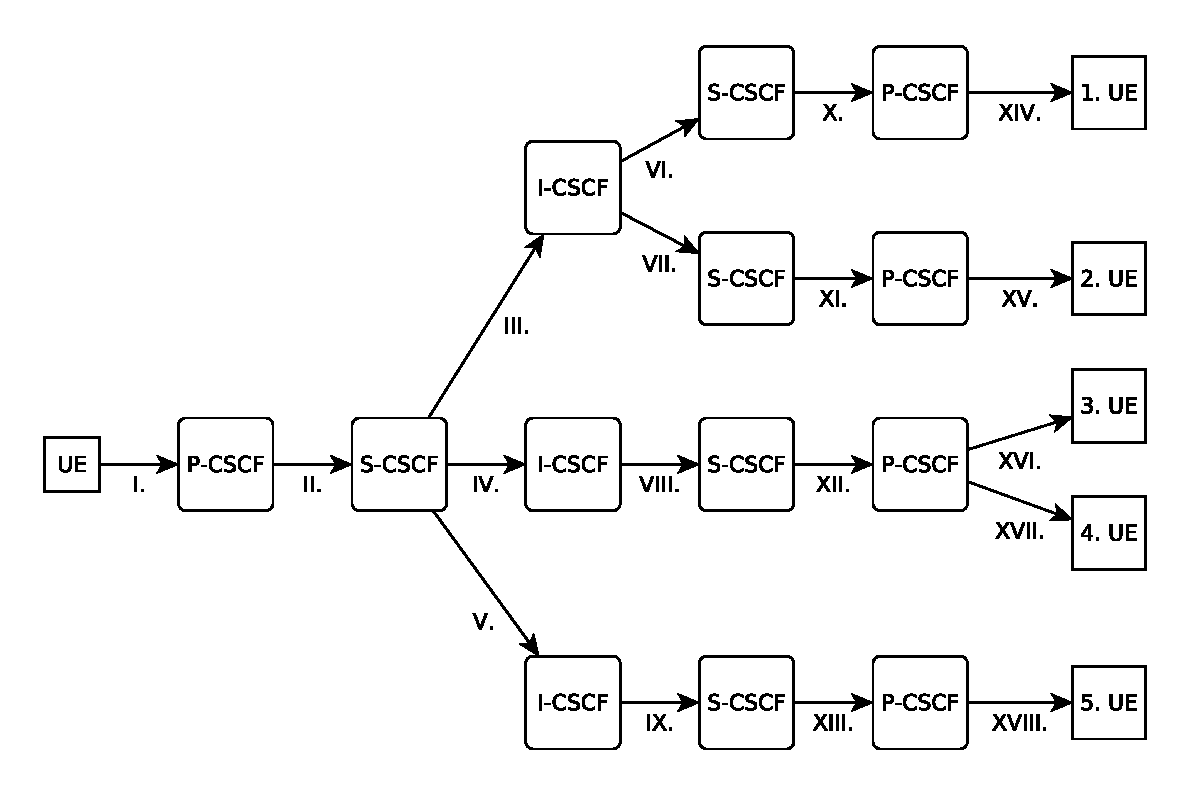
\includegraphics{img/MR-flow.eps}}
\caption{Az MR üzenetküldés folyamata}
\label{fig:mrflow}
\end{figure}

Mivel egy multimédia üzenet viszonylag nagy méretű is lehet, nagy valószínűséggel nem fér bele egyetlen MR üzenet törzsébe. Utóbbi probléma abból ered, hogy az IP hálózatokban maximalizálva van a hálózatba küldhető csomag mérete (MTU - Maximum Transmission Unit\footnote{IPV4-nél ez mekkora? Minimum 576 byte}). Hasonlóan a SIP MESSAGE üzeneteket használó megoldáshoz, itt is darabolni kellene a multimédia üzenetet több kisebb csomagra. Mivel az MR csomagok akár különböző útvonalon is eljuthatnak a címzettnek, a vételi oldalon való a csomagok eredeti sorrendjének visszaállíthatónak kell lennie. Amennyiben az MR üzenet fejlécében lehetőség lenne elhelyezni olyan mezőket, amelyek a helyes sorrend visszaállítását szolgálják, akkor a megoldás jelentősen jobb lenne, mint a SIP MESSAGE-et használó megvalósítás. Itt is általános feladatként jelentkezik a késleltett üzenetkézbesítés problémája, ami egy köztes alkalmazás szerver használatával megvalósítható lenne.

A vételi oldalon a kliensek, miután megkapták az MR kéréseket, nyugtázzák azokat. A cél itt is az, hogy a nyugták küldéséből eredő, a feladó és az őt kiszolgáló S-CSCF közötti linken folyó üzenetforgalmat minél jobban lecsökkentsük anélkül, hogy az IMS komponensek viselkedését alapvetően megváltoztatnánk. Ha a feladót kiszolgáló S-CSCF nem kompatibilis az MR üzenetekkel, akkor minden egyes nyugtát a hagyományos módon, egyesével továbbít a feladónak. Abban az esetben viszont, amikor az említett S-CSCF képes kezelni az MR üzeneteket, a hozzá beérkező, azonos típusú nyugtákra -- pl. 200 OK -- adott időtartamig vár, majd a nyugtákból összeállít egy MR választ, és csak ezt küldi el a feladónak, amivel jelentősen csökkenti a kérdéses link forgalmát.

\subsubsection{Üzenet továbbítása RTP protokoll segítségével -- {\color{red}IDE LEHET A VXML-es MRF-es megoldást kellene írni}}

{\color{red}Ezzel az a baj, hogy a video formátum erősen limitált. csak 3gp. Nem tudom, hogyan lehet képet átvinni. Ez főleg az interakciók miatt jó. max átvitt hang hossz is asszem limitált. Nem tudom, hogy erről kellene-e egyáltalán írni.}


\subsubsection{Üzenet továbbítása MSRP protokollal}
\label{sec:msrp_message}

Ez a megoldási javaslat a multimédia üzenetek felhasználók közötti átvitelére az MSRP (Message Session Relay Protocol) protokollt használja. Az MSRP -- a SIP-hez vagy a HTTP-hez hasonlóan -- egy szöveges, alkalmazás rétegbeli protokoll. A protokoll kapcsolat orientált adatátvitelt (session mode) tesz lehetővé, aminek számos előnye van a különálló, független üzenetcsomagok küldéséhez képest (paging mode).
Ezen előnyök közé tartozik, hogy a kommunikációs felek explicit felépítenek egymás között egy kommunikációs kapcsolatot az üzenet csomagok átvitelére. A kapcsolat léte magában foglalja többek között az összefüggő üzenet csomagok biztonságos, sorrendhelyes átvitelét, valamint a garantált kézbesítést is. Minden MSRP üzenet vagy egy kérés, vagy egy válasz. Az üzenetek fejlécből és törzsből állnak. A fejlécben az MSRP kapcsolatot, illetve a törzsben lévő -- szöveges vagy bináris -- tartalmat leíró információk találhatóak. Az MSRP kapcsolat felépítése SIP és SDP (Session Description Protocol) protokoll~\cite{rfc4566} segítségével történik. {\color{red} (IDE pár mondat az SDP-ről)} Az MSRP protokollról részletesebben az~\cite{rfc4975} irodalomban olvashat. 

Mivel a címzettek csoportjában lehet olyan felhasználó, aki az üzenet küldésének pillanatában nem elérhető, így a késletetett kézbesítés problémája ebben az esetben is felmerül. Utóbbi problémára itt is megoldást nyújt az, ha a kliensek közé egy alkalmazás szervert helyezünk el, amely többek között a késletetett üzenet kézbesítését is végzi. A köztes szerver használata a hálózati forgalmat is csökkenti, mivel a feladó és a szerver közötti, jellemzően alacsony sávszélességű (pl. rádiós) linken csak egyszer kerül átvitelre a -- gyakran nagy méretű -- multimédia üzenetet, szemben azzal az esettel, amikor a feladó minden címzettre külön-külön elküldi azt. Miután sikeresen átvitelre került a multimédia üzenet, a feladónak a címzettek listáját valamilyen módon, például egy SIP MESSAGE üzenet törzsében kézbesíteni kell a szerver felé. Mivel ez a lista jellemzően rövid szöveges üzenet, így belefér egyetlen SIP MESSAGE üzenetbe. A megoldás hátránya az MSRP kapcsolat felépítésének költsége, ami viszont a kapcsolat tényéből fakadó, már fentebb említett előnyökhöz képest elhanyagolható.

{\color{red} (... üzenet kézbesítés, előny, hátrány)}
\\
A dolgozatban a szolgáltatás fejlesztése során a fentebb leírt megoldások közül a legutolsó, MSRP protokollt használó megoldás használata mellett döntöttem. A SIP MESSAGE üzenetek használata nem célszerű \aref{sec:sip_message}.~fejezetben leírt számos hátránya miatt. \Aref{sec:mr_message}.~fejezetben tárgyalt MR üzenetet használó csoportos üzenetküldési megoldás jelenleg csak ajánlás formájában létezik, bárminemű szabványosítási eljárás jelenleg nincs folyamatban a témával kapcsolatban. Az MSRP protokollal való megvalósítás előnye a többi megoldási javaslattal szemben, hogy -- az IMS-ben jelen lévő --szabványosított eszközök használatára épít, illetve az adatátvitel kapcsolatorientált jellege következtében megbízható üzenetküldés valósítható meg. 

\subsection{Funkcionális terv}

A rendszer alapvetően a klasszikus kliens-szerver architektúrát valósítja meg. A kliensek azok, akik létrehozzák a multimédia üzeneteket, majd a szerver köz\-ve\-tí\-té\-sé\-vel elküldik azt kliensek egy meghatározott csoportjának. A szerver adatbázisban tárolja a multimédia üzenethez tartozó adatokat. A küldő kliens az átvitel si\-ke\-res\-sé\-gé\-ről folyamatos értesítést kap a szervertől. A szerver, miután sikeresen megkapta az új üzenetet, az online címzetteknek -- egy SIP MESSAGE üzenet törzsében -- azonnal értesítést küld erről. Az említett üzenet törzsének részletes ismertetése az {\color{red}xyz fejezetben} található. Egy kliens, amikor az új üzenetről értesítést kap a szervertől, a tényleges multimédia üzenetről kapott információk alapján eldöntheti, hogy érdekli-e őt az üzenet, vagy sem, és ezáltal a döntésnek megfelelő akciót végrehajtsa (azaz megtekintse a multimédia üzenetet vagy sem). 

A rendszer magasszintű modelljét \aref{fig:model}.~ábra szemlélteti.

\begin{figure}[htbp]
\center
\resizebox{10cm}{!}{
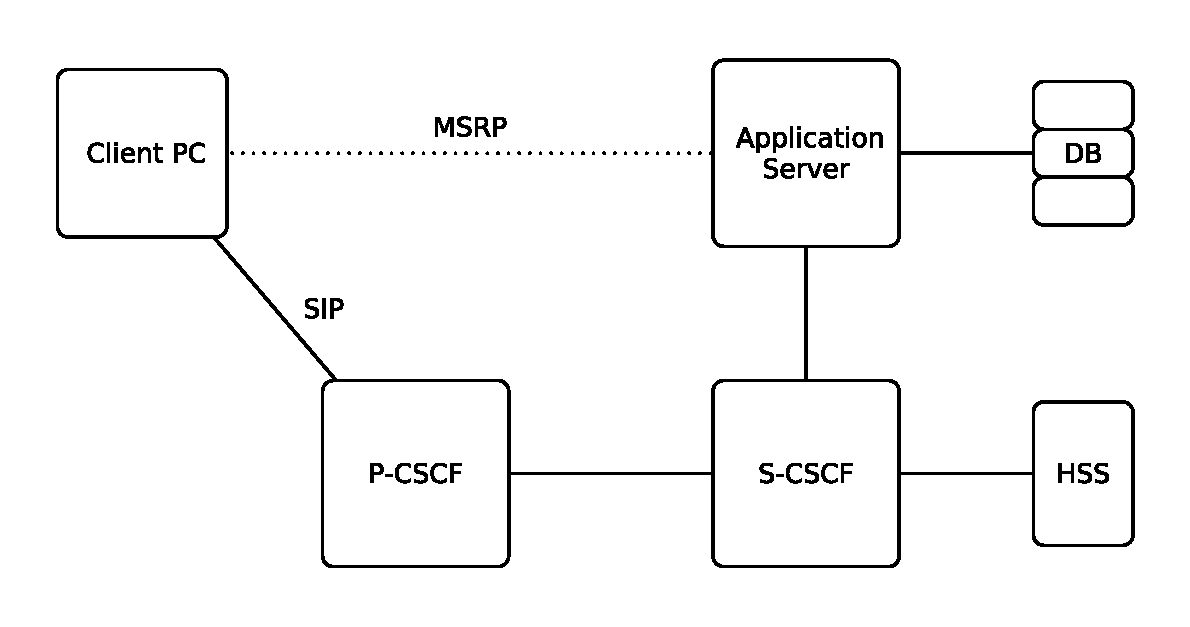
\includegraphics{img/system_MSRP_black.eps}}
\caption{A rendszer magasszintű modellje}
\label{fig:model}
\end{figure}

A rendszer az alábbi részekből épül fel:
\begin{mydescription}
\item[Kliens PC:] A felhasználó ezen keresztül éri el a szolgáltatást.
\item[Alkalmazás szerver:] Az üzenet fogadását és a címzetteknek való kézbesítést valósítja meg.
\item[Adatbázis szerver:] Az üzenethez tartozó adatok tényleges tárolását végzi.
\end{mydescription}

A következő fejezetekben az egyes elemek funkciójának részletes tárgyalása következik.

\subsubsection{Kliens}
\label{sec:kliens_pc}

A felhasználó ezen keresztül éri el az IMS hálózatot, azaz magát az üzenetküldő szolgáltatást is, ebből fakadóan a PC eszköznek rendelkeznie kell hálózati kapcsolattal. Miután a kliens oldali üzenetküldő szolgáltatást használó alkalmazás elindult, egy, a felhasználó SIP URI-ját tartalmazó üzenetet periodikusan elküld a szerver oldalnak. Ez a periodikus ,,regisztráció'' azért szükséges, hogy a szerver oldal, amikor új multimédia üzenetet kap egy felhasználótól, értesíteni tudja a címzettek közül azokat, akik aktuálisan elérhető állapotban vannak. 

A felhasználó multimédia üzenetet küldhet más, általa ismert felhasználók csoportjának. Az elküldendő multimédia üzenet többféleképpen állhat a kliens rendelkezésére. Egyik lehetséges opció, hogy az elküldenő üzenethez tartozó multimédia tartalom fájlrendszeren már a felhasználó rendelkezésére áll, kép, hang vagy videó fájl formájában. Ebben az esetben a küldő kliens fájlrendszeren való tallózással választhatja ki a multimédia tartalmat. A tartalom létrehozásának egy másik lehetséges módja, hogy a felhasználó a számítógépéhez kapcsolódó audiovizuális eszközökkel (mikrofon és kamera) maga készíti el a multimédia üzenethez tartozó kép, hang vagy videó felvételt. Miután az elküldendő multimédia üzenethez a tartalom a felhasználó rendelkezésére áll, valamilyen módon el kell küldeni a szerver oldalnak.

{\color{red}Ezeket inkább a megvalósítási tervbe kellene tenni. Vagy nem?}

Az üzenetküldés folyamatát \aref{fig:sending_proc}.~ábrán láthatjuk. A folyamat első lépéseként a küldő kliens és a szerver között fel kell építeni egy MSRP kapcsolatot, amelyen keresztül a multimédia üzenet átvitele történik. Egy MSRP kapcsolat minden esetben egy kliens és a szerver között épül fel, két kliens közvetlenül egymáshoz soha nem csatlakozik. Amikor az MSRP kapcsolat sikeresen felépült, a feladó ezen kapcsolaton keresztül MSRP csomagok\footnote{a szerkezetét hol lehetne leírni?} formájában továbbítja a multimédia üzenetet a szervernek. A szerver minden MSRP csomag vételét nyugtázza\footnote{nyugta formája} a küldő kliens felé. Miután a teljes üzenet sikeresen megérkezett a szerver oldalra, a a kliens bontja az MSRP kapcsolatot a szerverrel. A folyamat utolsó lépéseként a felhasználó egy SIP MESSAGE típusú üzenet törzsében elküldi a szervernek a címzettek listáját, illetve opcionálisan egyéb, az elküldött multimédia üzenetre jellemző információt. A címzett lista, illetve a kiegészítő információk XML (Extensible Markup Language) formátumban kerülnek átvitelre. Mivel az említett XML rövid, így az belefér egyetlen SIP MESSAGE üzenetbe. Miután a szerver sikeresen megkapta az XML-t tartalmazó üzenetet, a multimédia tartalommal együtt adatbázisban eltárolja azt, majd nyugtázza a sikeres vételt a feladó felé.

\begin{figure}[htbp]
\center
\resizebox{10cm}{!}{
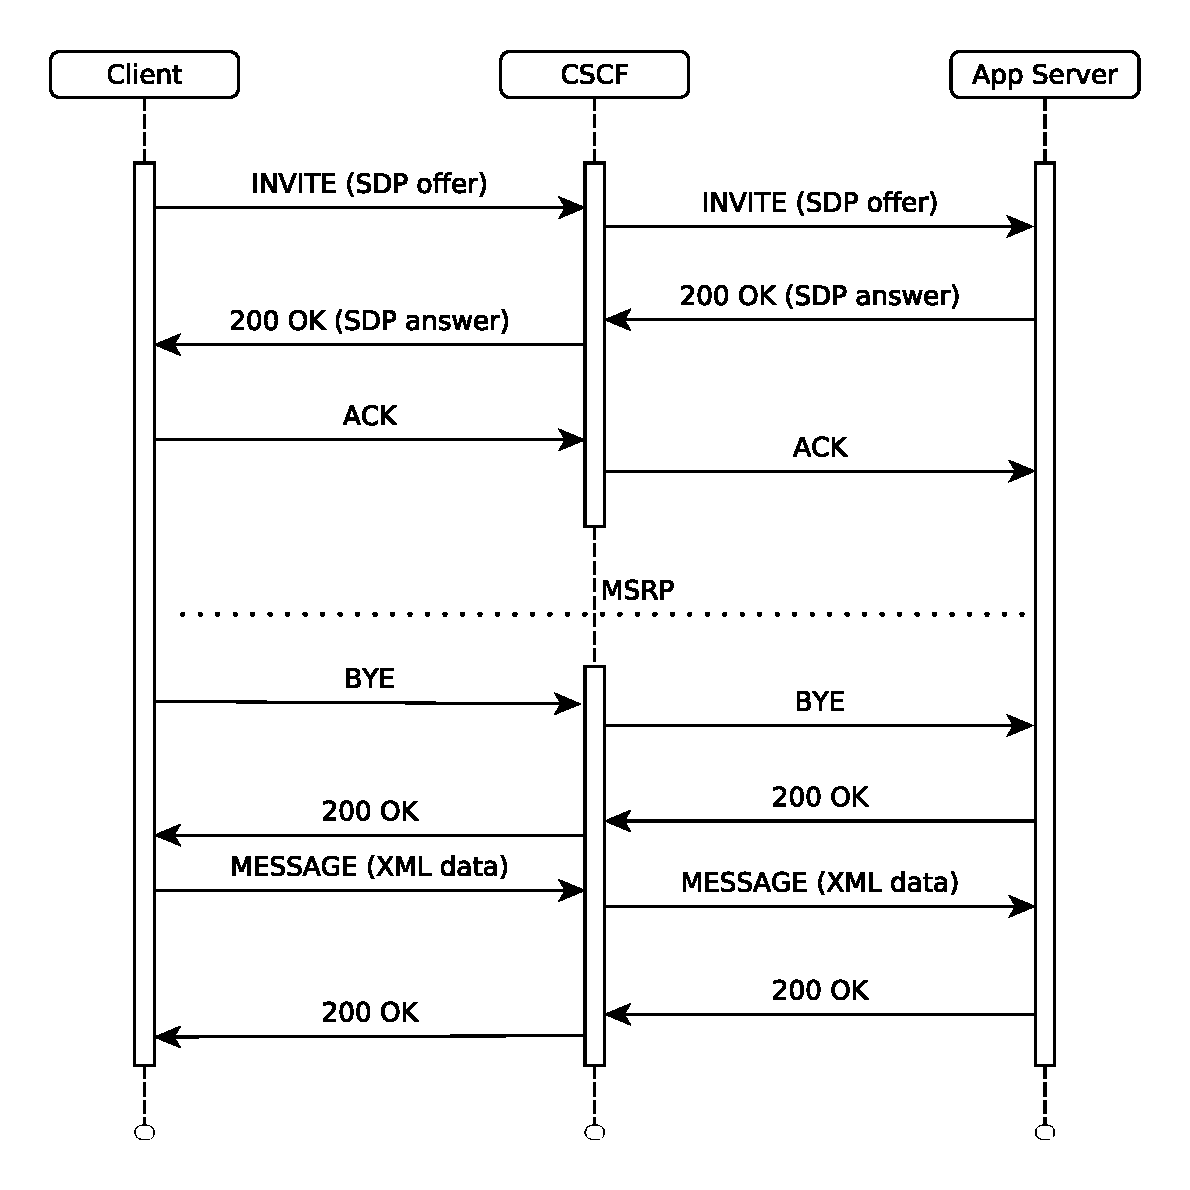
\includegraphics{img/sending_procedure.eps}}
\caption{Az üzenetküldés folyamata}
\label{fig:sending_proc}
\end{figure}

A kliens oldalon a multimédia üzenet vétele is több lépésben zajlik (\ref{fig:receiving_proc}.~ábra). Amennyiben a címzett felhasználó elérhető, úgy a szerver első lépésként egy SIP MESSAGE üzenetben értesíti a kliens oldalt a neki érkezett új multimédia üzenetekről. Utóbbi üzenet törzse szintén XML formátumban tartalmazza a multimédia üzenetekre jellemző adatokat. Második lépésként a kliens eldöntheti, hogy kiváncsi egy adott multimédia üzenetre, vagy sem. Amennyiben érdekli őt maga a multimédia tartalom is, felépít egy MSRP kapcsolatot a szerver oldallal, amelyen keresztül ,,letölti'' magát a tartalmat. A felhasználó dönthet úgy, hogy jelenleg nem kiváncsi az adott multimédia üzenetre. Utóbbi esetben nincs semmilyen további kommunikáció a kliens és a szerver között. A felhasználónak lehetősége nyílik egy adott multimédia üzenet tartalomátvitel nélküli törlésére is, ilyenkor szintén SIP MESSAGE üzenetben értesíti a szervert erről. Utóbbi esetben a multimédia üzenet törlődik a felhasználó szerver oldali postafiókjából.

\begin{figure}[htbp]
\center
\resizebox{10cm}{!}{
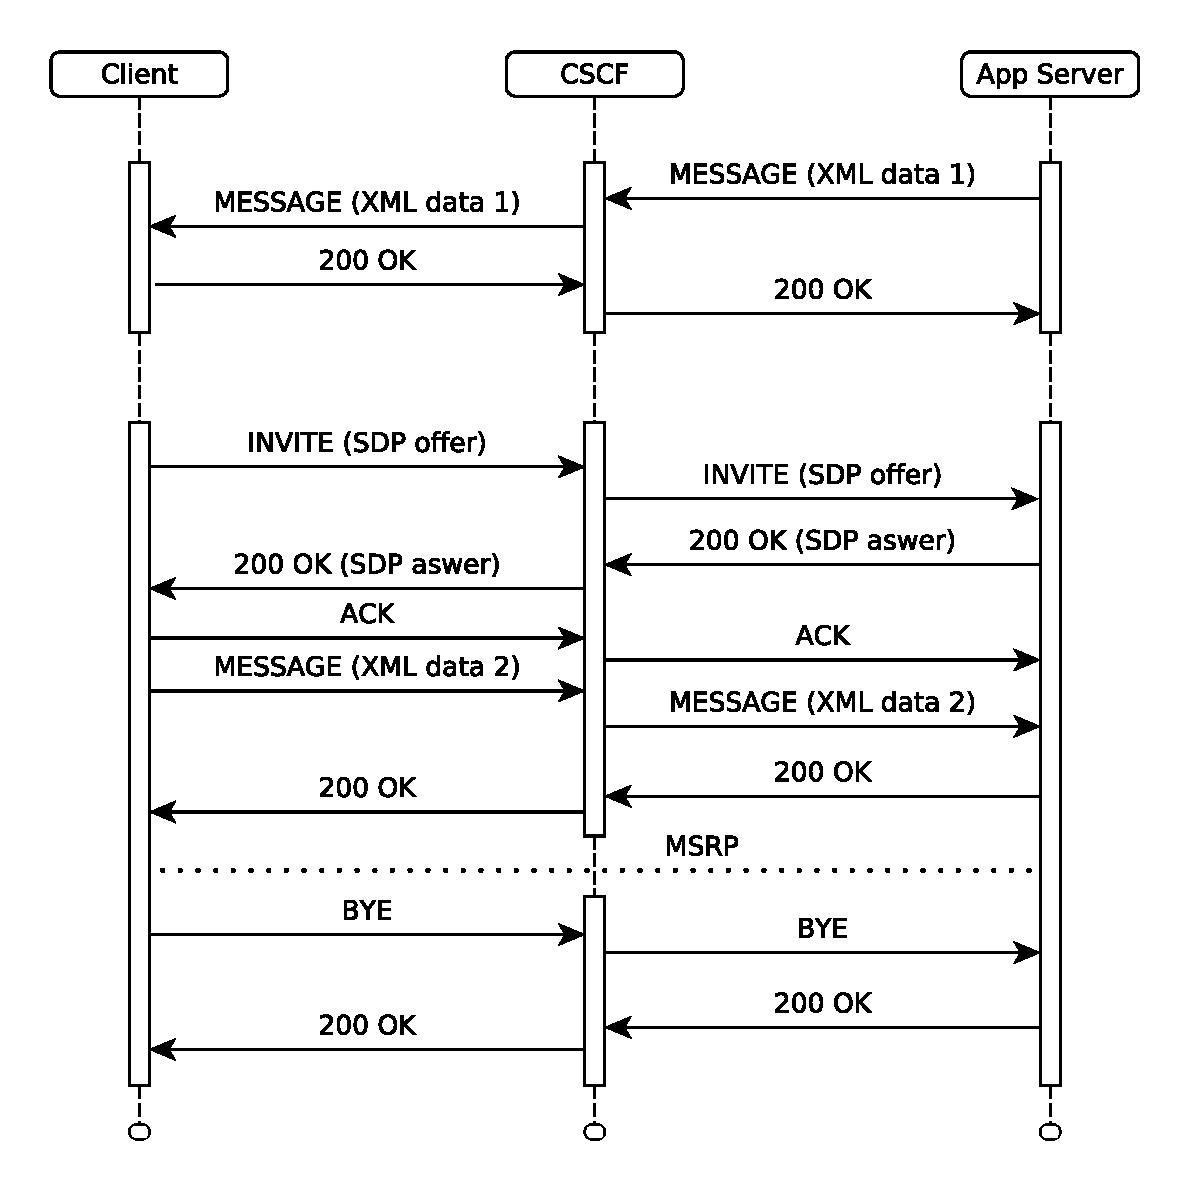
\includegraphics{img/receiving_procedure.eps}}
\caption{Az üzenet fogadás folyamata}
\label{fig:receiving_proc}
\end{figure}

\subsubsection{Alkalmazás szerver}
\label{sec:appserver}

Az alkalmazás szerver szolgáltatást nyújt a kliensek számára, az üzenetküldő rendszerben központi szerephet jut.

A szerver folyamatosan várja a kliensek csatlakozását. Miután a kliens oldali alkalmazás elindult, periodikusan értesíti a szervert arról, hogy elérhető a rendszerben. Amennyiben a periódusidő lejárta előtt a szerver nem kap újabb értesítő üzenetet egy klienstől, törli az adott felhasználót az elérhető kliensek listájából. 

A küldő kliens minden esetben az alkalmazás szerverrel építi fel a kapcsolatot, és annak küldi el a multimédia üzenetet. A szerver feladatai közé tartozik, hogy fogadja, majd adatbázisban eltárolja a feladótól érkező multimédia üzenetet, valamint az üzenethez kapcsolódó egyéb adatokat. Utóbbi adatok \aref{sec:kliens_pc}.~részben említett SIP MESSAGE üzenet törzsében XML formátumban érkeznek a kliens felől. Az XML a következő adatokat tartalmazza: 

\begin{itemize}\itemsep1pt
\item	A feladó SIP URI-ja
\item A címzettek SIP URI-jai
\item A üzenet azonosítója
\item Az üzenet tárgya
\item A multimédia tartalom formátuma
\end{itemize}

A szerver valósítja meg a késletetett üzenettovábbítást is. Utóbbi azt jelenti, hogy amikor a címzettek közül valamelyik nem elérhető, akkor az adott címzett értesítése az új üzenetről akkor történik meg, amikor az elérhetővé válik. Az értesítő üzenet -- hasonlóan a küldésnél használt üzenethez -- XML formátumban tartalmazza a multimédia üzenet adatait:

\begin{itemize}\itemsep1pt
\item	A feladó SIP URI-ja
\item A üzenet azonosítója
\item Az üzenet tárgya
\item A multimédia tartalom formátuma
\item A küldés dátuma
\end{itemize}

Az üzenet hatására a kliens oldal MSRP kapcsolaton a multimédia tartalom átvitelét kezdeményezheti, illetve az üzenet letöltés nélküli törlési igényét jelezheti. Az multimédia üzenet a tartalom sikeres átvitele után a szerver oldalon törlésre kerül a felhasználó fiókjából.

A kommunikáció során használt SIP MESSAGE üzenetek törzsében lévő XML tartalom szerkezetét \aref{sec:komm_uzenetek}.~fejezetben részletesen tárgyalom.

\subsubsection{Adatbázis szerver}
\label{sec:dbserver}

A küldő felhasználótól az alkalmazás szerveren keresztül érkező üzenetek átmeneti tárolását valósítja meg. Egy adott üzenethez tartozó adatok mindaddig adatbázisban tárolódnak, amíg a szerver az összes címzetthez sikeresen nem továbbította az üzenetet, vagy valamely címzettek nem jelezték az alkalmazás szerver felé, hogy ők nem kívánják megkapni az adott multimédia üzenet tényleges tartalmát. Az adatbázisban tárolásra kerülnek a feladótól érkező üzenet következő adatai:

\begin{itemize}\itemsep1pt
\item	A feladó SIP URI-ja
\item A címzettek SIP URI-jai
\item A üzenet azonosítója
\item Az üzenet tárgya
\item A multimédia tartalom
\item A multimédia tartalom formátuma
\item A küldés dátuma
\end{itemize}

\subsection{Üzemeltetési terv}
\label{sec:uzemeltetesi_terv}

Ide talán jöhetne use-case diagram, annak leírása... Vagy nem kell? Minden, ami ide jönne, már le van írva máshol is. 

\subsection{Interfész terv}
\label{sec:interfesz_terv}

Az egyes modulok közötti interfészek leírása...

Két fő komponensre különül el a rendszer fejlesztése: kliens-
ill. szerveroldali részre.

\subsubsection{Kliens}
\label{sec:kliensinterfesz}

\subsubsection{Szerver}
\label{sec:szerverinterfesz}

\subsection{Adatbázis terv}

A következő fejezetek a kommunikációs üzenetek szerkezetét, valamint a használt adatbázis felépítését tárgyalják.

\subsubsection{Kommunikációs üzenetek}
\label{sec:komm_uzenetek}

\subsubsection{Az adatbázis}
\label{sec:adatb}

\subsection{Megvalósítási terv}
\label{sec:megvalositas}

Ide jönnek majd az állapotgépek, működés leírása...

\subsubsection{A kliens megvalósítása}
\label{sec:kliensmegvalositas}

\subsubsection{A szerver megvalósítása}
\label{sec:szervermegvalositas}


\subsection{Összefoglalás}

